% ----------------------------------------------------------
% Histórico dos tipos de aplicações
% ----------------------------------------------------------
\chapter[Fundamentos]{Fundamentos}
%\addcontentsline{toc}{chapter}{Histórico}
% ----------------------------------------------------------

\section{IPC - Interprocess Communication}\label{sec:ipc}


Diversos sistemas operacionais fornecem mecanismos para viabilizar a comunicação e o compartilhamento de dados entre aplicações. Coletivamente, as atividades habilitadas por estes mecanismos são chamadas de interprocess communications (IPC) \cite{microsoft-ipc}.

Nem sempre um programa sequencial é a melhor solução para um determinado problema. Muitas vezes, as implementações são estruturadas na forma de várias tarefas inter-dependentes que cooperam entre si para atingir os objetivos da aplicação \cite{sistemas-op-mazierro}.

Os mecanismos que garantem a comunicação entre processos concorrentes e os acessos aos recursos compartilhados são chamados \textit{interprocess communication}. Algumas formas de IPC facilitam a divisão de trabalho entre diversos processos especialistas, enquanto outras  facilitam esta divisão entre computadores dentro de uma rede.

Normalmente, os aplicativos que fazer parte de uma comunicação através de IPC são categorizados como clientes ou servidores. Um cliente é um aplicativo ou um processo que solicita um serviço de alguma outra aplicação ou processo. Por outro lado um servidor é um aplicativo ou um processo que responde a uma solicitação de cliente. Muitas aplicações agem como um cliente e um servidor, dependendo da situação \cite{microsoft-ipc}.

A figura \ref{fig:how-communication-works} mostra como ocorre a comunicação entre processos (P1 e P2). Esta troca de informação pode acontecer de duas maneiras: em duas etapas, ou de forma direta. A comunicação em duas etapas envolve um processo coordenador, que pode ser um interpretador em Python utilizado para dar início ao \textit{workflow} por exemplo. A comunicação direta é ilustrada na figura ligada por linhas pontilhadas e não necessita de intermediação de nenhum processo. Esta maneira de comunicação pode ser executada através de diversas formas, entre elas: Pipes, Shared Memoty, Mapped Memory e Arquivos compartilhados.

\begin{figure}[ht]
    \centering
    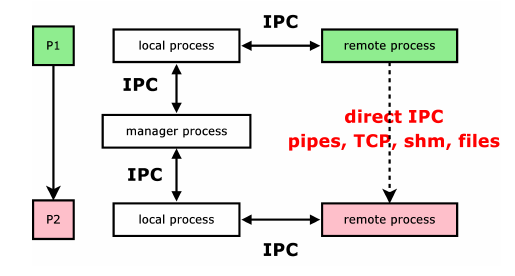
\includegraphics[width=1\textwidth]{figuras/ipc.png}
    \legend{Características dos mecanismos de comunicação \citeonline{sistemas-op-mazierro}}
    \label{fig:how-communication-works}
\end{figure}

\section{Cliente/Servidor}\label{sec:clientserver}

Também conhecido como arquitetura de duas camadas, o modelo cliente/service consiste em uma arquitetura em que a camada de apresentação se encontra no cliente e a camada de dados esta armazenada no servidor. Esta separação se opõe ao modelo centralizado amplamente utilizado.

O processamento dos dados é dividido em duas partes distintas. Uma parte é a requerente de dados (cliente), e a outra parte é a provedora dos dados (servidor). O cliente envia durante sua execução uma ou mais solicitações ao servidor para realizar alguma tarefa específica. É delea responsabilidade tanto de apresentar as informações para o usuário, quando executar as regras de negócio necessárias à aplicação. O servidor é responsável por armazenar os dados e prover um meio para que o cliente os consulte.

Desde a década de 1990, fornecedores de software desenvolvem e trazem ao mercado muitas ferramentas para simplificar o desenvolvimento de aplicativos para a arquitetura cliente/servidor de 2 camadas. Algumas das mais conhecidas são: Microsoft Visual Basic, Delphi da Borland e PowerBuilder da Sybase. Essas ferramentas combinadas com milhões de desenvolvedores que sabem usá-las, significa que a abordagem de duas camadas de cliente/servidor é uma solução econômica para certas classes de problemas.

Desde então, aplicações \textit{desktop} comunicando-se com o servidor de banco de dados era um caso de uso normal. A maior parte da lógica de negócios foi incorporada dentro da aplicação \textit{desktop}. Portanto, esse estilo de aplicativos cliente/servidor também foi chamado de \textit{fat clients}. 

\begin{figure}[ht]
    \centering
    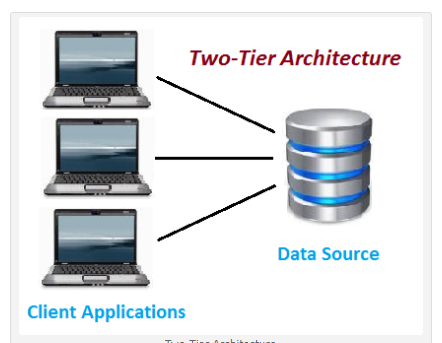
\includegraphics[width=0.5\textwidth]{figuras/two-tier.png}
    \caption{Comunicação em duas camadas}
    \label{fig:two-tier}
\end{figure}

A figura \ref{fig:two-tier} ilustra como a arquitetura em duas camadas funciona, mantendo uma comunicação direta entre cliente e servidor, sem intermediarios entre as duas pontas. Visto que neste modelo as regras de negocio estão presentes na camada de aplicação, ele é frequentemente aplicado em ambientes homogêneos. A camada de banco de dados e a camada de aplicação estão fisicamente próximos, o que oferece um bom desempenho para as aplicações.

Por outro lado, o modelo cliente servidor em duas cadamas possui grandes desafios de escabilidade. Quando multiplos usúarios executam requisições simultaneas, a aplicação perde muito desempenho, dado ao fato que cada cliente precisa de conecções separadas e memória de CPU para processar as requisições. Entretando, um dos maiores problemas na arquitetura em duas camadas ocorre quando há mudanças na estrutura do banco de dados. A maioria das aplicações usadas para interação depende da estrutura do banco de dados criando um problema quando é preciso remodela-lo, já que as aplicações são dependentes da estrutura predominante.

Esta modelo foi substituido pelo modelo de tres ou n camadas, muito mais eficiente, e amplamente utilizado nas aplicações atuais [ESCREVER MAIS SOBRE ISSO]

\section{Aplicações Monolíticas}\label{sec:monolitico}

Conforme \citeonline{monolithic-definition} explica, uma aplicação monolítica é construída como uma única unidade de \textit{software}. As aplicações empresariais são construídas em três partes: um banco de dados (que consiste em tabelas geralmente em um sistema de gerenciamento de banco de dados), uma interface de usuário do lado do cliente (consistindo de páginas executando em um navegador ou aplicativos móveis) e um lado do servidor aplicação. Este aplicativo do lado do servidor tratará as requisições HTTP, executará a regra de negócio, recuperará e atualizará dados do banco de dados e construirá as respostas para serem enviadas às aplicações clientes. Estas camadas representam uma aplicação monolitica - um único executável lógico. Para fazer alterações no sistema, é necessário criar e implantar uma versão atualizada do aplicativo do lado do servidor.

Uma aplicação monolítica é autônoma e independente de outras aplicações. A filosofia do projeto consiste em um aplicativo que não é responsável apenas por uma determinada tarefa, mas que também pode executar todos os passos necessários para completar uma determinada função, como é mostrado na figura \ref{fig:three-tier}.

\begin{figure}[ht]
    \centering
    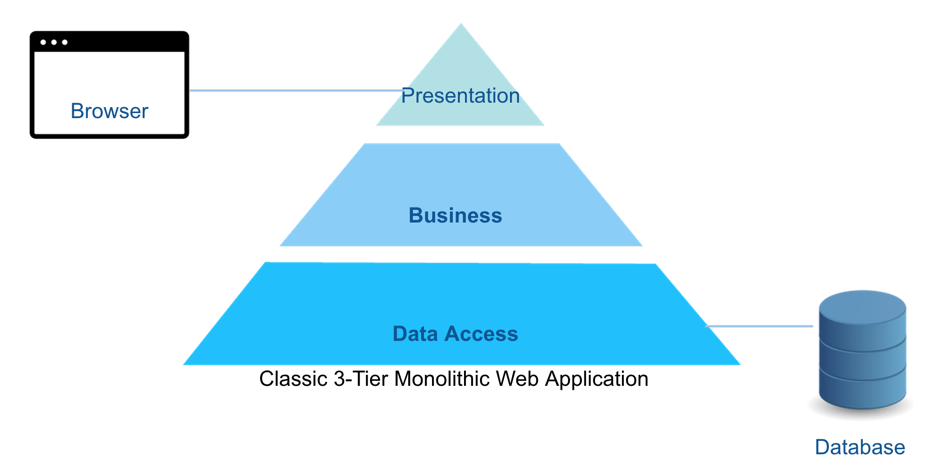
\includegraphics[width=0.5\textwidth]{figuras/three-tier.png}
    \caption{Aplicação monolítica clássica em 3 camadas}
    \label{fig:three-tier}
\end{figure}

\citeonline{monolithic-extinction} afirma que as aplicações monolíticas são uma maneira natural para a evolução de uma aplicação. A maioria das aplicações começam com um único objetivo, ou um pequeno número de objetivos relacionados. Ao longo do tempo, novas funcionalidades são adicionados ao aplicativo para suportar as necessidades do negócio. 

Temos alguma desvantagens nos sistemas moniliticos, alguns deles são: 

\begin{itemize}
    \item Um único ponto de falha pode comprometer o funcionamento correto de todos os módulos do sistema.
    \item Baixa estalabilidade dado a necessidade de copiar toda a \textit{stack} para escalar horizontalmente.
    \item Base de código \textbf{gigante}, uma vez que toda a regra de negócio se encontra em uma só base.
    \item É necessário muita comunicação para que várias equipes de desenvolvedores trabalhem em paralelo. Esta sobrecarga diminui o ritmo de desenvolvimento.
\end{itemize}

Contudo, com a popularização dos \textit{frameworks} Javascript como Angular e Backbone, houve um movimento de desacoplação da camada de visualização nas aplicações monoliticas. Foram criadas então as chamadas aplicação \textit{frontend}, responsáveis pela camada de apresentação, e sendo executadas em dispositivos móveis como \textit{smartphones} e \textit{tables} ou nos \textit{browsers desktop}. 

Esse movimento criou um modelo monolítico de duas camadas, ilustrado na figura \ref{fig:two-tier-monolithic}. A remoção da interdependência entre as cadas de interface e servidor de aplicação facilitou o escalonamento e a escalabilidade de cada uma das partes. Esta separação de conceitos foi o primeiro passo em direção a uma arquitetura orientada a serviços.

\begin{figure}[ht]
    \centering
    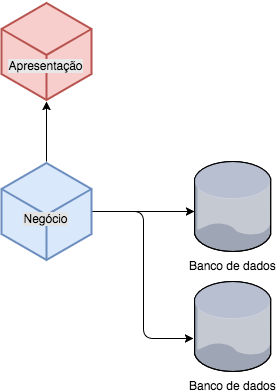
\includegraphics[width=0.5\textwidth]{figuras/two-tier-monolithic.png}
    \caption{Modelo monolítico de duas camadas}
    \label{fig:two-tier-monolithic}
\end{figure}

\section{SOA - Service Oriented Architecture}\label{sec:soa}

\citeonline{soa-cbdi} define SOA como políticas, práticas e frameworks que permitem que rotinas de aplicações sejam fornecidas e consumidas como conjuntos de serviços publicados em uma granularidade relevante para o consumidor do serviço. Os serviços podem ser invocados, publicados e descobertos e são abstraídos da implementação usando uma única forma de interface baseada em padrões.

Além de criar e expor serviços, \citeonline{soa-tech-target} assinala que o SOA tem a capacidade de aproveitar esses serviços uma e outra vez em aplicativos (conhecidos como aplicativos compostos). A SOA vincula esses serviços à orquestração ou alavanca individualmente esses serviços. Assim, a SOA é realmente sobre como consertar arquiteturas existentes, abordando a maioria dos principais sistemas como serviços e resgatando esses serviços em um único domínio onde eles são formados em soluções.

 O SOA permite a reutilização de ativos existentes, onde novos serviços podem ser criados a partir de uma infra-estrutura de sistemas de TI existente. Em outras palavras, ele permite que as empresas alavancem os investimentos existentes, permitindo que eles reutilizem aplicativos existentes e possibilita a interoperabilidade entre aplicações e tecnologias heterogêneas. SOA fornece um nível de flexibilidade que não era possível antes, no sentido de que:

\begin{itemize}
    \item Os serviços são componentes de software com interfaces bem definidas que são independentes da implementação. Um aspecto importante da SOA é a separação da interface de serviço (o que) da sua implementação (como). Esses serviços são consumidos por clientes que não estão preocupados com a forma como esses serviços irão executar seus pedidos.
    \item Os serviços são autônomos (executar tarefas predeterminadas) e vagamente acoplados (para independência)
    \item Serviços compostos podem ser construídos a partir de agregados de outros serviços
\end{itemize}

Isso significa que o SOA é uma abordagem alinhada com o negócio em que os aplicativos dependem dos serviços disponíveis para facilitar os processos de negócios. Um serviço é um componente de software reutilizável autônomo fornecido por um provedor de serviços e consumido pelos solicitantes de serviço. O SOA cria uma visão de flexibilidade de TI que facilita a agilidade do negócio. A implementação de uma SOA envolve principalmente componentes de aplicativos corporativos e/ou em desenvolvimento que usam serviços, disponibilizando aplicativos como serviços para outras aplicações \cite{soa-book}.

\begin{figure}[ht]
    \centering
    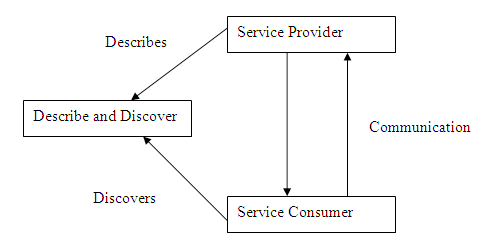
\includegraphics[width=0.5\textwidth]{figuras/soa.png}
    \caption{Service Oriented Architecture}
    \label{fig:soa}
\end{figure}

\citeonline{soa-intel} acrescenta que em um ambiente SOA típico, existe um provedor de serviços e um consumidor de serviços. Para que isso funcione, também precisa de um mecanismo para que eles possam se comunicar uns com os outros, como  é ilustrado na figura \ref{fig:soa}.  A W3C \footnote{World Wide Web Consortium} definiu um padrão aberto para que \textit{web services} possam implementar SOA e habilitar a comunicação entre o provedor e o consumidor atravém de um protocolo baseado em XML o Simple Object Access Protocol (SOAP). Outros padrões também são usandos ou foram criados para realizar a comunicações entre os serviçoes SOA. Alguns basearam-se no \textit{design} do REpresentation State Transfer (REST), utilizando tanto XML quando JSON para transportar os dados entre os serviços. 

There seems to be general confusion about the relationship between SOA and Web services. In an April 2003 Gartner report, Yefim V. Natis makes the distinction as follows: "Web services are about technology specifications, whereas SOA is a software design principle. Notably, Web services' WSDL is an SOA-suitable interface definition standard: this is where Web services and SOA fundamentally connect." Fundamentally, SOA is an architectural pattern, while Web services are services implemented using a set of standards; Web services is one of the ways you can implement SOA. The benefit of implementing SOA with Web services is that you achieve a platform-neutral approach to accessing services and better interoperability as more and more vendors support more and more Web services specifications.